\documentclass[dvips,12pt]{article}

\usepackage[pdftex]{graphicx}
\usepackage{subcaption}
\usepackage{float}
\usepackage{url}
\usepackage[utf8]{inputenc}
\usepackage{geometry}
\usepackage{setspace}
\usepackage{amsmath}
\usepackage{txfonts}

% From amsmath, prepend equation numbers with section number
%\numberwithin{equation}{section}

% graphicx: Where should graphics be found?
\graphicspath{ {figures/} }
\graphicspath{{./figures/}} % allows figures to be placed in a different folder

% Setup margins and paper size
\geometry{
  letterpaper,
  total={170mm,257mm},
  left=20mm,
  top=20mm,
  bottom=25mm
}



%\title{ECEN 773 Project: Planar VTOL}
%\author{Jesse Wynn}
%\date{April 20, 2017}

\begin{document}

\begin{titlepage}

\begin{center}

\vspace*{\fill}

\vspace{0.5in}

% Insert your title here
{ \LARGE \bfseries LQR Control of a Planar VTOL}\\[.25in]

\large
by\\[.25 in]
% Change your name here
Jesse Wynn\\[1in]

Final Project for ECEN 773--Linear Systems Theory \\
Brigham Young University \\

\vspace{1in}

\today

\vspace*{\fill}

\end{center}

\end{titlepage}

\section{Introduction}
For this project an LQR controller was implemented on a simple MIMO linear system.  The dynamic system that was chosen to model and control was a simple two-dimensional UAV, or planar VTOL.  The planar VTOL seemed to be an ideal system to study since it is relatively simple, yet it has many similarities to more complex rotor-craft systems such as quadrotor UAVs.  In Dr. Beards undergraduate controls class, the planar VTOL was used as an ongoing case-study exercise, and this project is an extension of that work.  The specifics of this project include re-modeling the linear system as a single complete state-space system, and then implementing LQR control, set-point control, and observer-based control in MATLAB and SIMULINK.  

\section{Linear Dynamic Model}

The planar VTOL is characterized by a point mass $m_c$ at the vehicle center, and two additional point masses $m_l$ and $m_r$ at a distance $d$ on opposite sides of the vehicle.  The term $m_c$ represents the vehicle's main body and electronics, and $m_l$ and $m_r$ represent electric motors and propellers.  There are three forces acting on the VTOL which are $f_l$, $f_r$, and then the force of gravity $f_g$.  The vehicle pose is defined by horizontal displacement $z$, angle $\theta$, and vertical displacement $h$. An illustration is given below.

\begin{figure}[h] %  figure placement: here, top,  bottom, or page
   \centering
   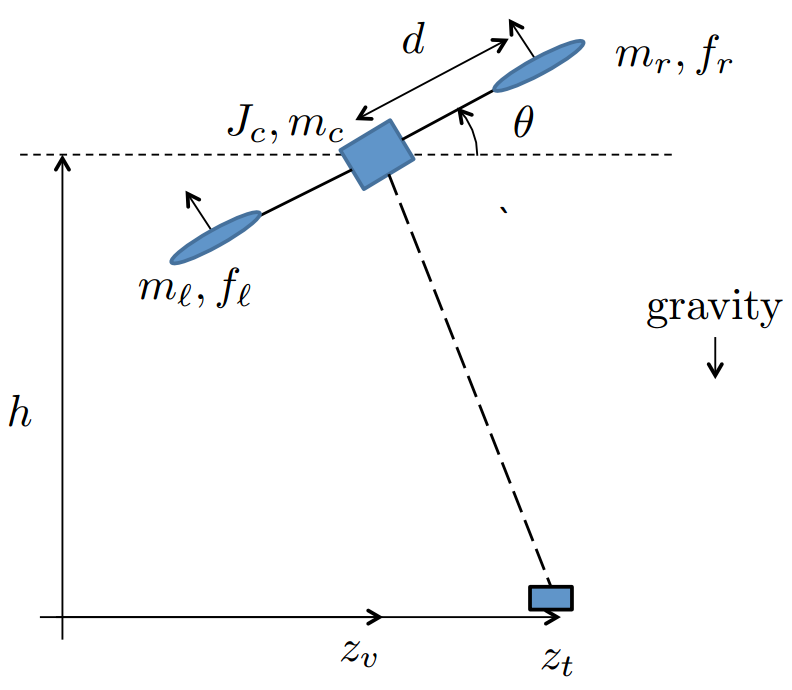
\includegraphics[trim = 0mm 0mm 0mm 0mm,clip,width=3in]{planar_vtol.png}
   \caption{Planar VTOL physical System Definition}
   \label{fig:vtol}
\end{figure}

The dynamic model (or plant) that is used in simulation includes the full non-linear dynamics of the VTOL.  For the controls design however, a much simpler linear model is used. Using principles of linearization from the textbook, the linear dynamics of the system were found to be

\begin{equation}
\ddot{z} = \frac{-F_e\theta}{m_c + 2m_r}  + \frac{-\mu\dot{z}}{m_c + 2m_r}
\end{equation}

\begin{equation}
\ddot{\theta} = \frac{\tau}{J_c + 2m_r d^2}
\end{equation}

\begin{equation}
\ddot{h} = \frac{\tilde{F}}{m_c + 2m_r}
\end{equation}

where $F_e$ is an equilibrium force to counteract gravity, $\mu$ is a damping force to represent the propeller drag, $J_c$ is the VTOL's rotational moment of inertia, and $\tau$ and $\tilde{F}$ capture the combined force and torque from $f_l$ and $f_r$. These linear dynamics can be put into state-space form as follows:



{\begin{gather}
 \dot{x}
 =
 \begin{bmatrix}
     \dot{z} \\
     \dot{\theta} \\
     \dot{h} \\
     \ddot{z} \\
     \ddot{\theta} \\
     \ddot{h} \\
   \end{bmatrix}
   =   
   \begin{bmatrix}
        0 & 0 & 0 & 1 & 0 & 0  \\
        0 & 0 & 0 & 0 & 1 & 0 \\
        0 & 0 & 0 & 0 & 0 & 1 \\
        0 & \frac{-F_e}{m_c + 2m_r} & 0 & \frac{-\mu}{m_c + 2m_r} & 0 & 0 \\
        0 & 0 & 0 & 0 & 0 & 0 \\
        0 & 0 & 0 & 0 & 0 & 0 \\
      \end{bmatrix}
      \begin{bmatrix}
           z \\
           \theta\\
           h \\
           \dot{z} \\
           \dot{\theta} \\
           \dot{h} \\
         \end{bmatrix}
         +
         \begin{bmatrix}
                    0 & 0\\
                    0 & 0\\
                    0 & 0\\
                    0 & 0\\
                    \frac{1}{J_c + 2m_r d^2} & 0\\
                    0 & \frac{1}{m_c + 2m_r}\\
                  \end{bmatrix}
                  \begin{bmatrix}
                                      \tau \\
                                      \tilde{F} \\
                                    \end{bmatrix}           
\end{gather}}
{\begin{gather}
 y
 =
 \begin{bmatrix}
     1 & 0 & 0 & 0 & 0 & 0\\
     0 & 1 & 0 & 0 & 0 & 0\\
     0 & 0 & 1 & 0 & 0 & 0\\
   \end{bmatrix}
      \begin{bmatrix}
           z \\
           \theta\\
           h \\
           \dot{z} \\
           \dot{\theta} \\
           \dot{h} \\
         \end{bmatrix}
         +
		 \begin{bmatrix}
		            0 & 0 \\
		            0 & 0 \\
		            0 & 0 \\
		          \end{bmatrix}
		          \begin{bmatrix}
		                         \tau \\
		                         \tilde{F} \\
		                     \end{bmatrix}      
\end{gather}}

\section{Full-State Feedback LQR}

With the state-space representation of our system formed, the first step in implementing the LQR controller was to verify that the system was controllable.  Using MATLAB, the controllability matrix $ \mathcal{C} $ was computed and checked to see if it was full-rank.  In our case it was, and we proceed to set up our $Q$ and $R$ matrices.  $Q$ and $R$ were initialized as identity and then tuned from there to get good response from the system.  In the end, $Q$ and $R$ ended up as:

\begin{center}
$
 Q
 = 
   \begin{bmatrix}
        1 & 0 & 0 & 0 & 0 & 0  \\
        0 & 1 & 0 & 0 & 0 & 0 \\
        0 & 0 & 200 & 0 & 0 & 0 \\
        0 & 0 & 0 & 2 & 0 & 0 \\
        0 & 0 & 0 & 0 & 1 & 0 \\
        0 & 0 & 0 & 0 & 0 & 500 \\
      \end{bmatrix}
      \quad
      R
       = 
         \begin{bmatrix}
              1 & 0  \\
              0 & 1  \\
            \end{bmatrix}         
$
\end{center}
The optimal gain $K$ for the VTOL system was then found using MATLAB's \textit{lqr(A,B,Q,R)} function.  Implementing the full-state feedback LQR controller consisted of defining the basic control law of $u = -Kx$ where $u$ is the input to the plant or, and $x$ is the state vector.  To test the LQR controller, the VTOL was initialized a small distance away from \textit{zero} and the response was observed (see Figure ~\ref{fig:stepresp}).  As can be seen from the step response, the LQR controller does good job of regulating the VTOL $z$-displacement and $h$-displacement to \textit{zero}. 


\begin{figure}
\centering
\begin{minipage}{.5\textwidth}
  \centering
  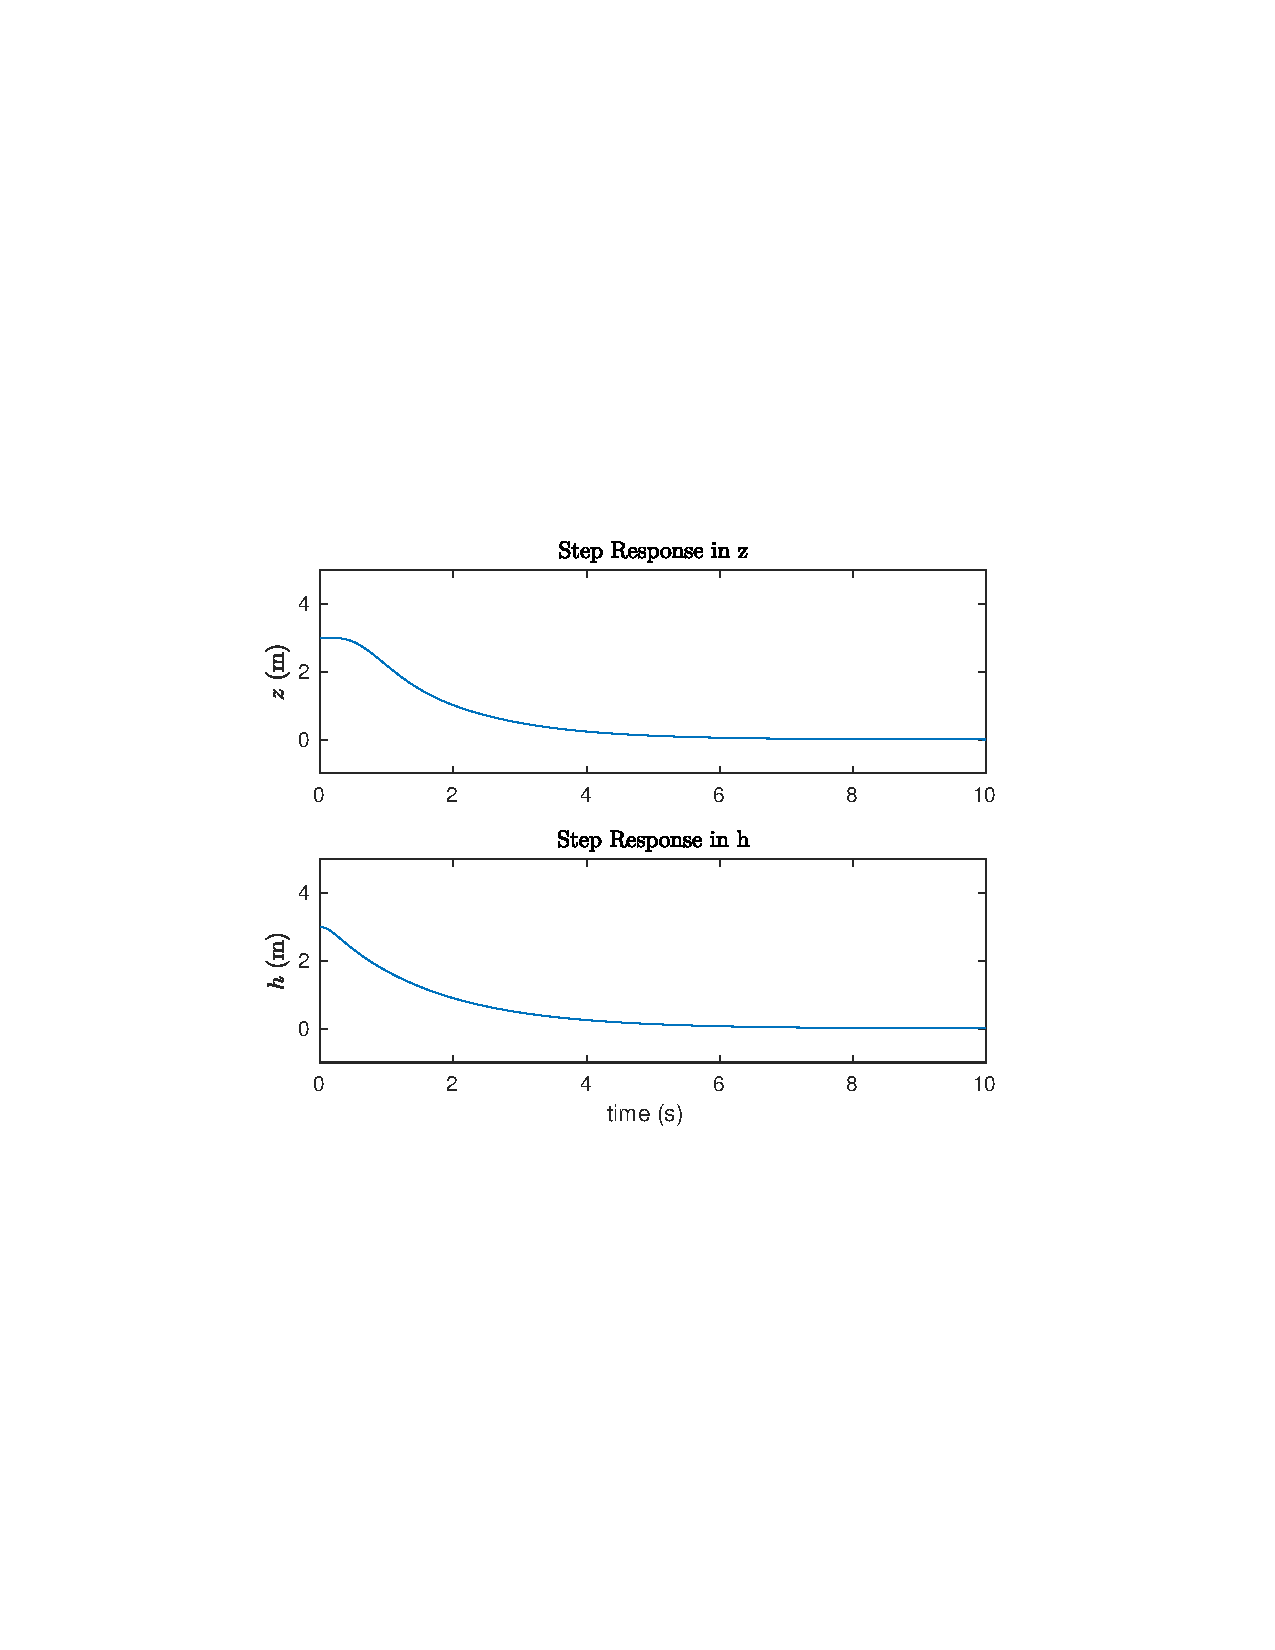
\includegraphics[trim = {4cm 8.75cm 4cm 9cm},clip,width=3in]{step_response.pdf}
  \captionof{figure}{VTOL step response under LQR}
  \label{fig:stepresp}
\end{minipage}%
\begin{minipage}{.5\textwidth}
  \centering
  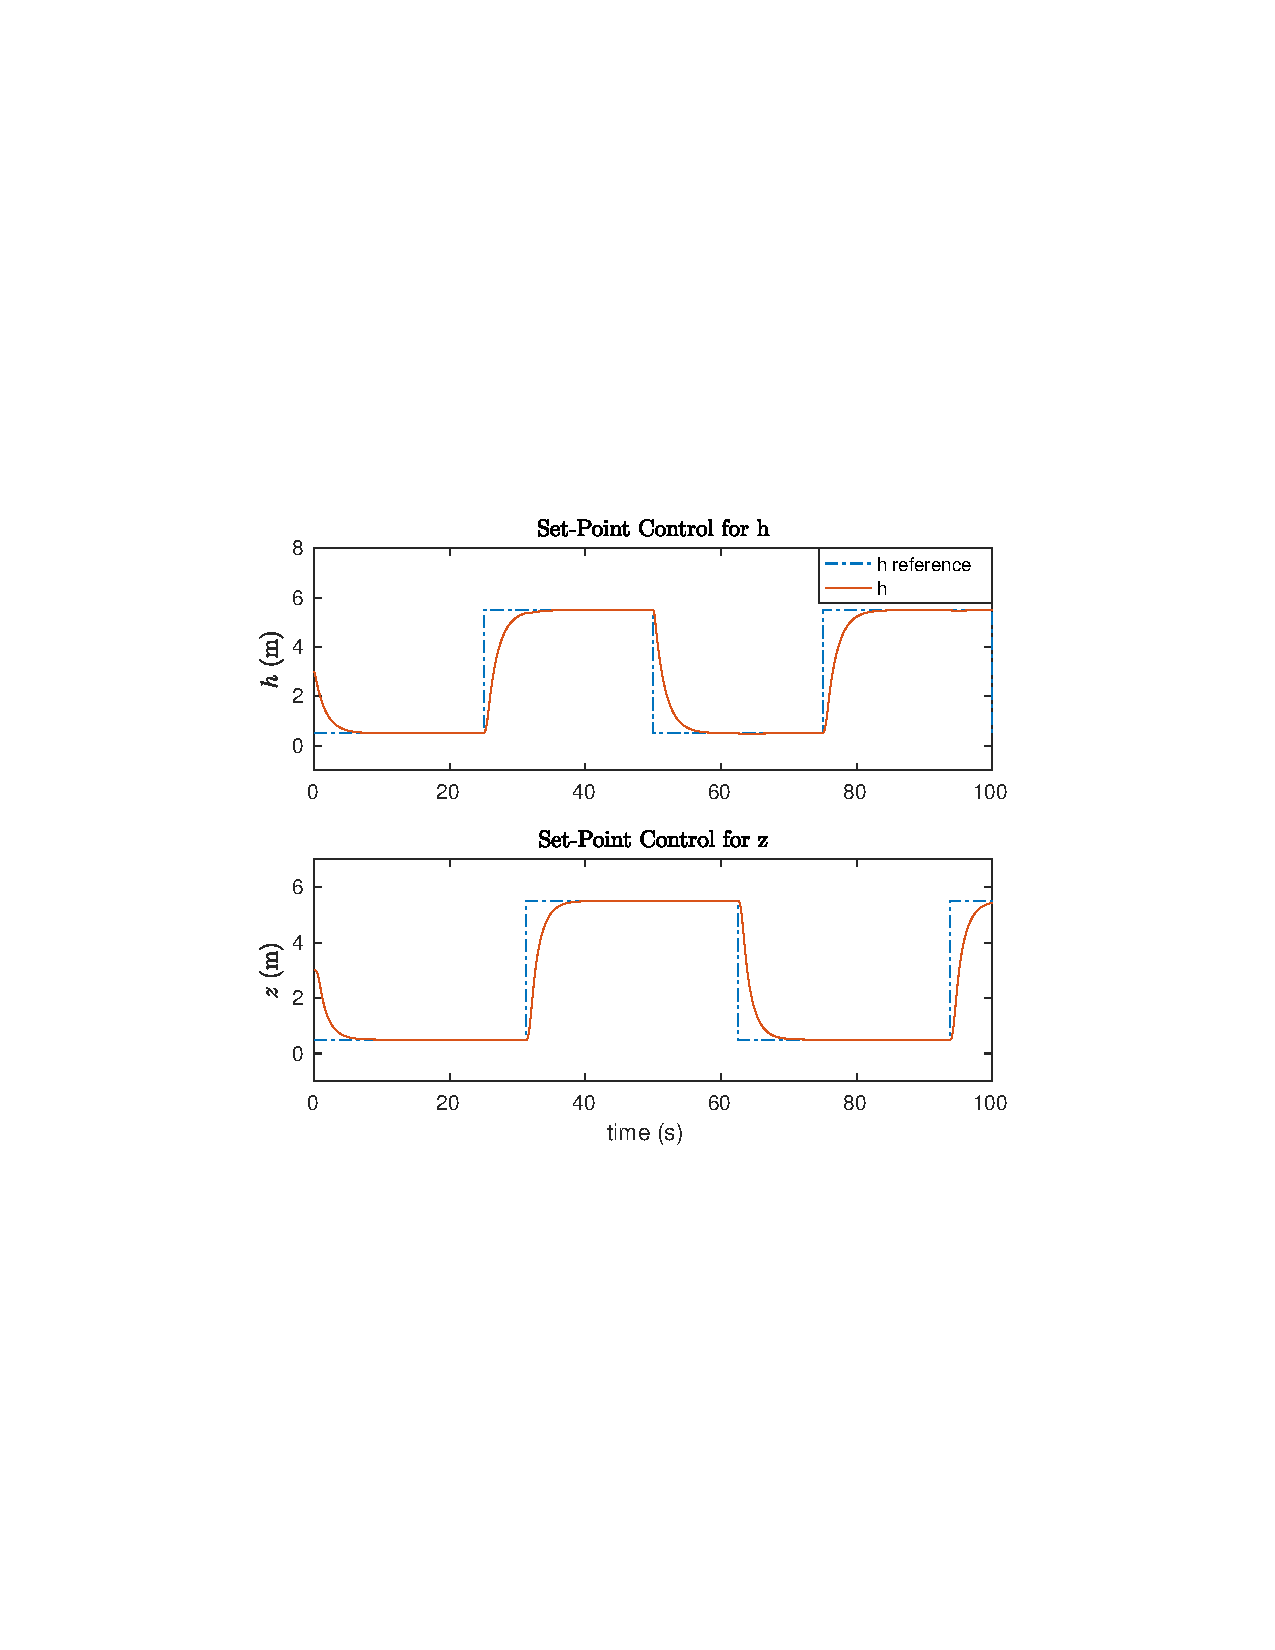
\includegraphics[trim = {4cm 8.5cm 4cm 8.5cm},clip,width=3in]{set_point.pdf}
  \captionof{figure}{VTOL set-point LQR control}
  \label{fig:setpoint}
\end{minipage}
\end{figure}

\section{Set-Point LQR Controller}

With the LQR controller working well as a state-regulator, the next step was to implement a simple set-point LQR controller.  To do this, the control law was modified slightly to be $u = -K(x-x_r)$ where $x_r$ was a desired reference state. In this case $x_r = \begin{bmatrix} z_r & 0 & h_r & 0 & 0 & 0 \end{bmatrix}^\intercal$ with $z_r$ and $h_r$ being the desired displacement values. The result of the set-point controller with square waves for $z_r$ and $h_r$ can be seen in Figure ~\ref{fig:setpoint}.

\section{Adding an Integrator}

A downside of the LQR controller by itself is that if the actual system parameters differ from those used to model the system, or if there are unknown disturbances such as wind, then there will be steady-state offset between the reference and the actual state.  To solve this problem, one option is to add an integrator to the closed-loop system.  In the case of the VTOL, an integrator was added by modifying the control law to be $u = -K(x-x_r) + k_i(error)$.  The integrator was tested by changing the mass of the VTOL and adding a small amount of wind in the $z$-direction.  The effectiveness of the integrator is shown in Figure ~\ref{fig:integrator}. Note that the steady-state error is removed.

\begin{figure}[h]
\centering
\begin{subfigure}{.5\textwidth}
  \centering
  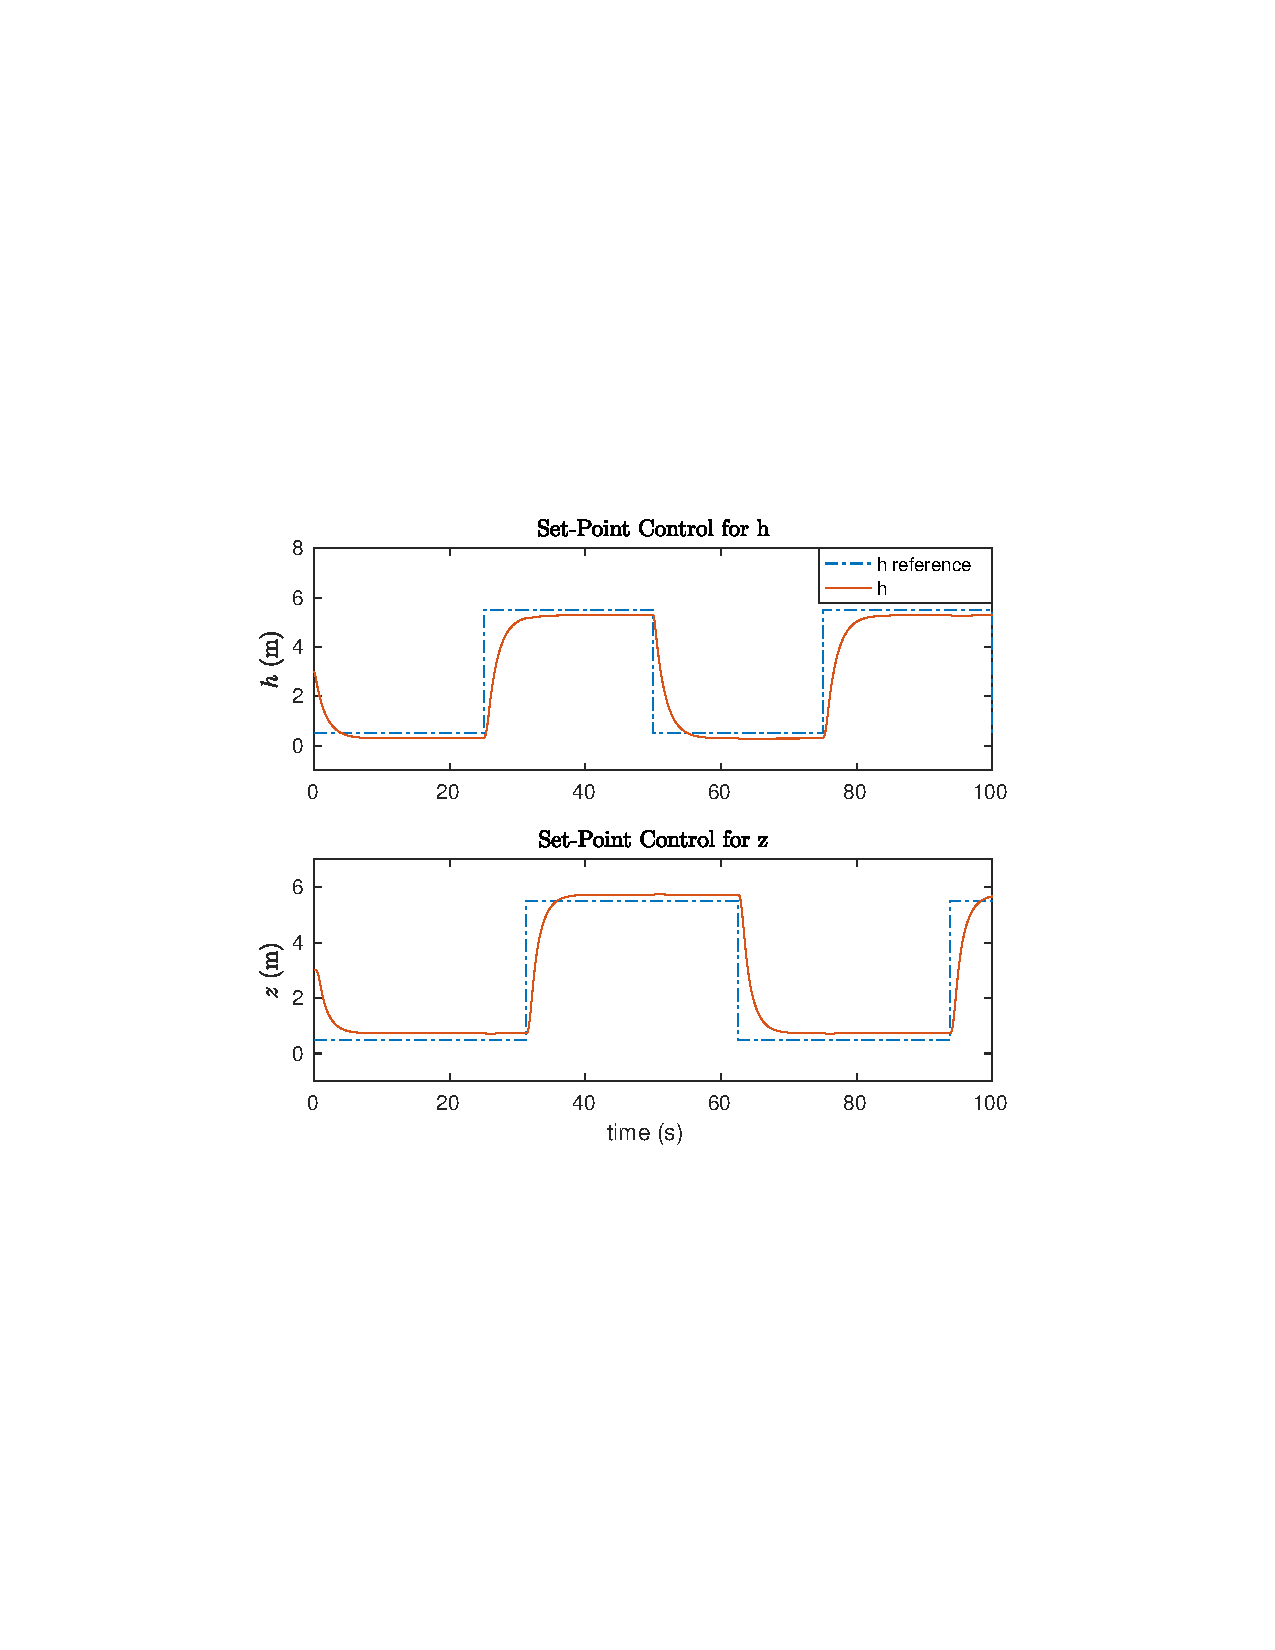
\includegraphics[trim = {4cm 8.5cm 4cm 8.5cm},clip,width=3in]{set_point_no_int.pdf}
  \caption{Disturbances present with no integrator}
  \label{fig:sub1}
\end{subfigure}%
\begin{subfigure}{.5\textwidth}
  \centering
  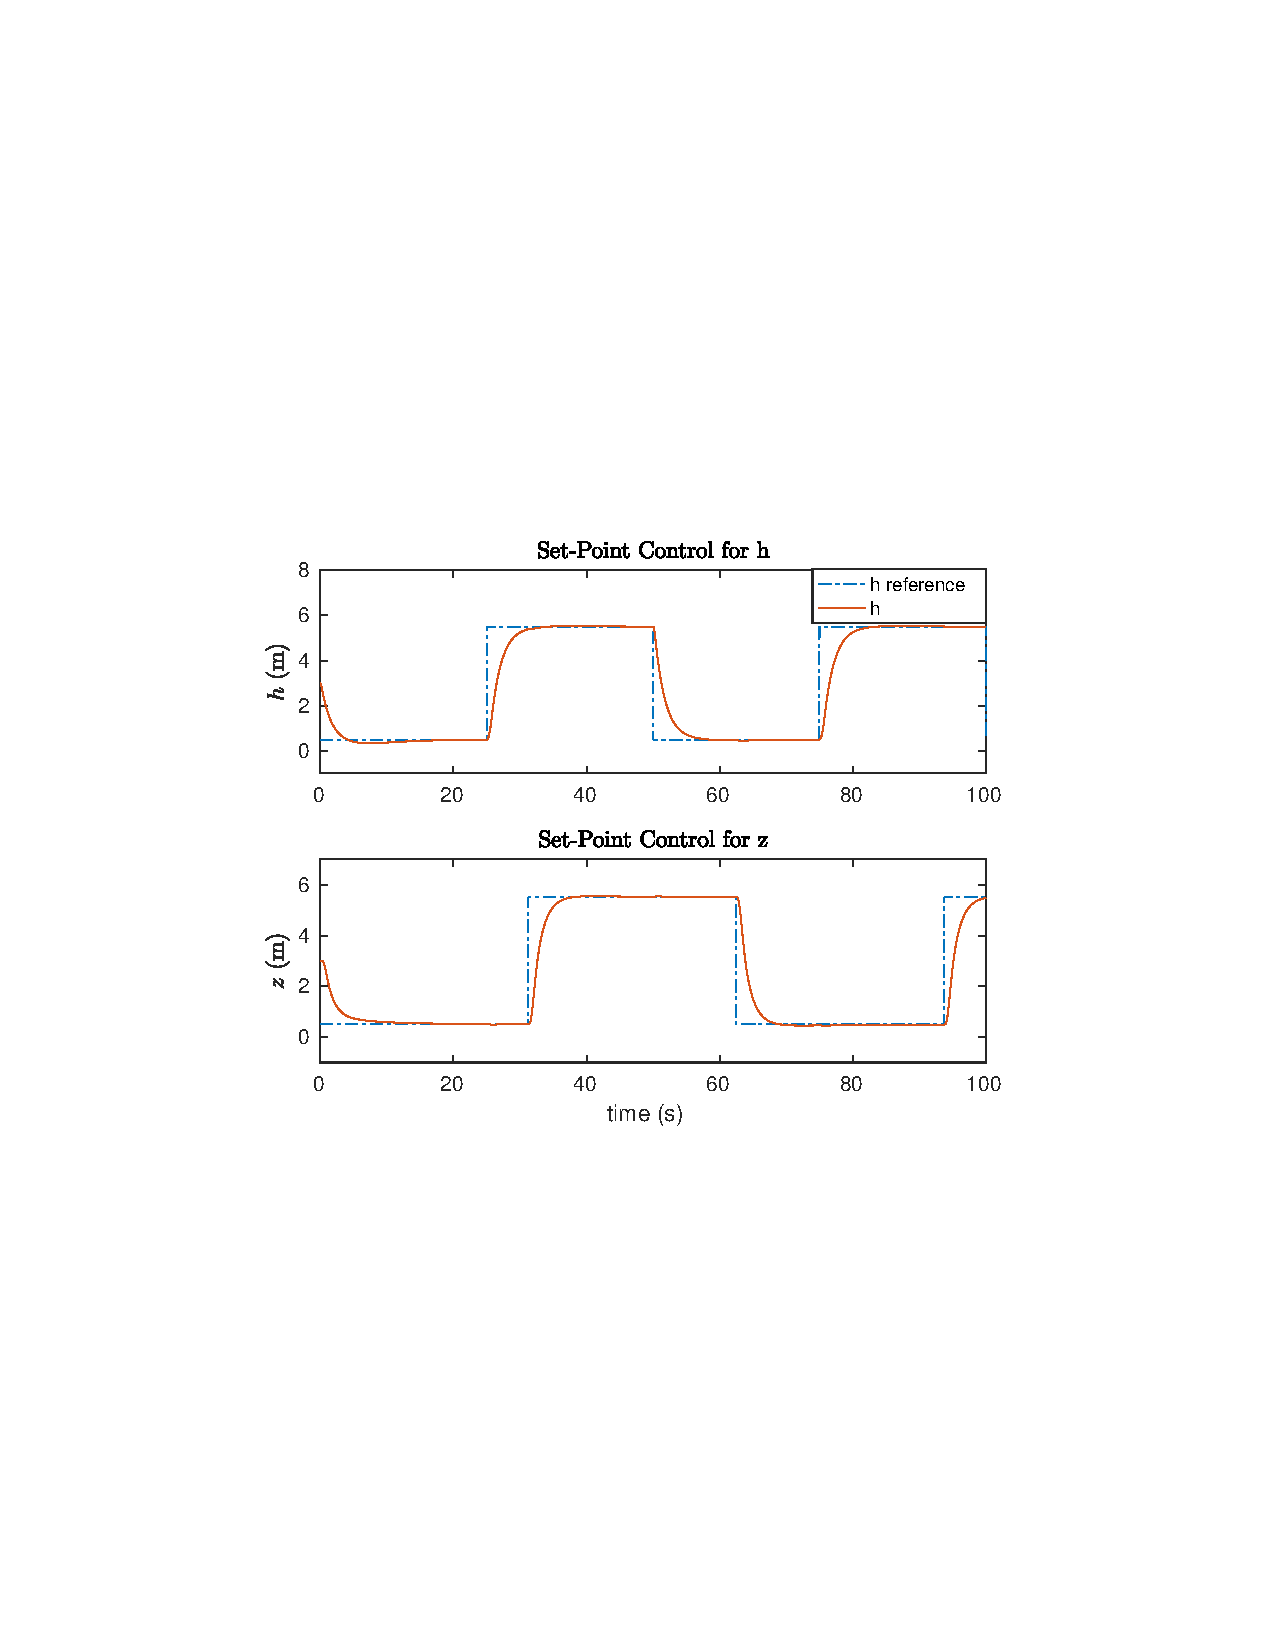
\includegraphics[trim = {4cm 8.5cm 4cm 8.5cm},clip,width=3in]{set_point_w_int.pdf}
  \caption{Disturbances present with Integrator added}
  \label{fig:sub2}
\end{subfigure}
\caption{Adding an integrator to remove steady-state offset}
\label{fig:integrator}
\end{figure}


\section{Implementing an Observer}

For almost all real dynamic systems, assuming full-state feedback is unrealistic.  In many systems only the output portion of the state can be measured.  When this is the case, a simple state estimator called an observer can be implemented to generate an estimated state $\hat{x}$. The full derivation of the observer dynamics is absent in this work, but the result of adding an observer to the closed-loop system can be represented by the following state-space equations:

{\begin{gather}
 \begin{bmatrix}
     \dot{x} \\
     \dot{e} \\
   \end{bmatrix}
   =   
   \begin{bmatrix}
        A-BK & BK  \\
        0 & A-LC  \\
      \end{bmatrix}
      \begin{bmatrix}
           x \\
           e \\
         \end{bmatrix}
         +
         \begin{bmatrix}
                    B \\
                    0 \\
                  \end{bmatrix}
                  r         
\end{gather}}
{\begin{gather}
   y
   =   
   \begin{bmatrix}
        C & 0  \\
      \end{bmatrix}
      \begin{bmatrix}
           x \\
           e \\
         \end{bmatrix}
         +
         \begin{bmatrix}
                    0 \\
                  \end{bmatrix}
                  r         
\end{gather}}
Here $K$ is the optimal gain found previously with $L$ being the observer gain.  For the our system, the observer poles were chosen to be about 10-times larger than the corresponding open-loop poles of the VTOL.  This ensures that the observer can keep up and reliably generate a good state estimate $\hat{x}$.  Once the observer poles had been set, and thanks to the duality between $A$ and $A^\intercal$, and $B$ and $C^\intercal$,  the observer gain $L$ could be computed using the MATLAB \textit{place()} command.
\end{document}

%\begin{figure}
%\centering
%\begin{subfigure}{.5\textwidth}
%  \centering
%  \includegraphics[width=.4\linewidth]{image1}
%  \caption{A subfigure}
%  \label{fig:sub1}
%\end{subfigure}%
%\begin{subfigure}{.5\textwidth}
%  \centering
%  \includegraphics[width=.4\linewidth]{image1}
%  \caption{A subfigure}
%  \label{fig:sub2}
%\end{subfigure}
%\caption{A figure with two subfigures}
%\label{fig:test}
%\end{figure}
